\section{CrashSimulator Approach Details}

    \begin{figure*}[t]
        \center{}
        \fbox{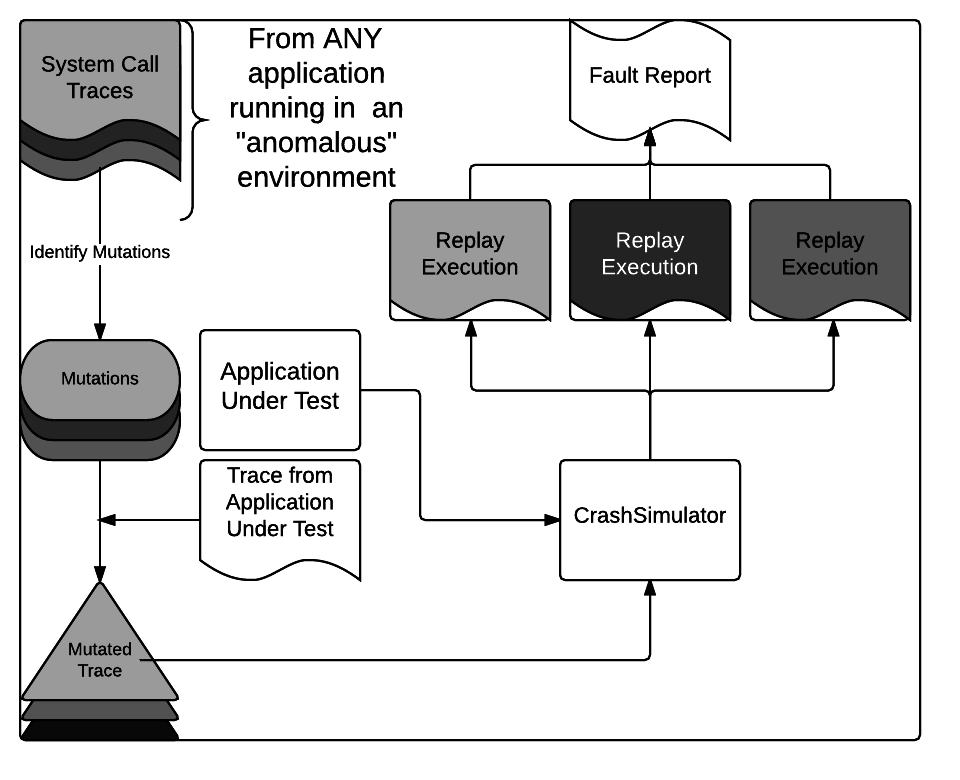
\includegraphics[scale=.5]{Architecture}}
        \caption{CrashSimulator Architecture}
    \end{figure*}

    \subsection{Architecture}

        At a high level CrashSimulator is organized into three primary modules. The first module is responsible for
        interpreting the input system call traces and identifying opportunities to inject faults into the application
        under test. The second module's primary purpose is producing mutated versions of the input ``clean'' system call
        trace. The specific mutations it makes are based on the anomalies identified during analysis of the input system
        call traces. The final module is responsible for iterating through the set of anomalous system call traces in
        order to test each one of them. For each anomalous trace, this module launches a test instance of the
        application under test and replays the anomalous system call trace. During this process, it monitors the
        application's behavior and reports any faults.

        The test launcher was separated from the test controller for the sake of portability. A great deal of the test
        launcher's code deals with the low level details of process manipulation and monitoring and, as such, will
        likely require modification in order to operate on different platforms than the authors' original development
        environments. For example, in order to modify the return value of particular system calls on x86 systems, the
        test launcher must hook the application under test using \emph{ptrace} and modify the values of the EAX register
        upon completion of the system call. This modification is tightly coupled to x86 calling conventions. Even the
        relatively similar x86--64 differs in that the test launcher must use \emph{ptrace} to modify the RAX register
        rather than the EAX register. Other architectures, such as ARM, will likely require more extensive
        modifications.

        All three primary CrashSimulator modules are packaged together and interact with each other at the appropriate
        times without user intervention. At this point, CrashSimulator itself is available as a virtual machine
        appliance compatible with the \emph{Virtual Box} virtual machine hosting software. The reasons for distributing
        CrashSimulator in this manner are threefold. First, this distribution method ensures that all of
        CrashSimulator's dependences are installed and configured appropriately. Second, this method provides an
        environment for taking system call traces that is known to be complete tool-wise and compatible with
        CrashSimulator. Finally, and most importantly, this method provides an environment that is known to be
        compatible with the low level details of CrashSimulator's fault injection techniques.

        CrashSimulator's source code is available and, while other environments may be untested, it should function
        correctly on any platforms that meet the criteria described above.

    \subsection{Anomaly Identification}

        The first step in CrashSimulator's operation is the analysis of the set of input system call traces recorded
        from other applications running in the intended deployment environment. These traces can be taken from any
        application that as environmental requirements that are reasonably similar to the application under test. For
        example, a web server could likely be effectively tested by CrashSimulator when CrashSimulator is given system
        call traces from other applications that make heavy use of the network. Testing a web browser with traces from
        an application that has no network usage at all would result in less effective testing.

        CrashSimulator was designed to accept identified anomalies from any tool that can output them in the proper
        format. In this implementation, CrashSimulator was written to accept the output of NetCheck. NetCheck readily
        able to identify a wide variety of anomalous behaviors related to network communication between one or more
        hosts. During normal operation, NetCheck analyzes a group of input system call traces and attempts to produce a
        diagnosis for network related faults. When operating as an anomaly identification tool for CrashSimulator its
        operation remains the same. Adapter code in CrashSimulator allows the normal output from NetCheck to be consumed
        without any modifications to NetCheck itself. This output is used to derive the mutations that will be made to
        the application under test's ``ideal'' system call trace in order to induce the faults NetCheck identified in
        the applications that yielded the input system call traces.

    \subsection{System Call Traces}

        Where other tools base their operation of direct analysis of the application under test CrashSimulator operates
        based on information gleaned from system call traces. This gives CrashSimulator several advantages over similar
        tools. First, CrashSimulator operates in a language independent manner. It can test any program given two
        conditions hold true:

        \begin{enumerate}
            \item{The application can run in the testing environment}
            \item{System call traces can be recorded from from applications similar to the application under test while
                they run in the intended deployment environment}
        \end{enumerate}

        Utilizing system call traces provides CrashSimulator with two advantages over similar tools. First,
        CrashSimulator has no need for complex language parsing and analysis code. It can test an application regardless
        of the programming language it was written in. Second, while other tools focus on the application under test in
        isolation, CrashSimulator is able to extensively test the interfaces between the application under test and its
        environment. This means that faults resultant from these interfaces are readily identified. For example,
        existing tools are able to quickly test for flaws that result from improper parsing of data once it
        has been received from across a network. CrashSimulator is able to induce and identify flaws that result from
        improper behavior during the network communication itself. This second type of flaw is much more difficult to
        identify replicating the application's intended deployment environment or deploying the application and testing
        it live.

        % TODO: Rework from here down

    \subsection{Potential Deviations}

        \textbf{I would really like to find another term besides anomaly}

        CrashSimulator's goal when analyzing a normal run system call trace is to identify individual system calls or
        patterns of system calls that it recognizes as an opportunity to inject a fault during subsequent runs. These
        signatures are referred to as ``potential anomalies.'' CrashSimulator has the ability to identify and classify
        anomalies into the following categories.

        \subsubsection{Return Value Modification}

            One way CrashSimulator can inject faults into the running application is to modify the return values of
            interesting system calls identified in the previous trace analysis step. The primary driver behind injecting
            this type of fault is the tendency of developers to misuse common API functions or misunderstand their
            failure modes. The \emph{recv} system call, for example, returns the number of bytes of data it was able to
            copy into the requested buffer from the specified socket. A developer that is unfamiliar with the operation
            of \emph{recv} may assume that a positive return value means that \textbf{all} of the requested data was
            successfully copied. This assumption fails to account for cases where the system call completed successfully
            but copied less data than the developer was expecting. A well written application might make repeated calls
            to recv until it has gathered all the data it needs while an incorrectly written application may only call
            it once resulting in a fault when it tries to process incomplete data in the future.

            % TODO: Make sure terminology is correct in this paragraph
            % TODO: Is this methodology reasonable?
            The authors' implementation of CrashSimulator injects this fault using ptrace. The application under test is
            executed in a process that is hooked by ptrace and each system call made by the application is examined.
            When a system call that was previously identified as a target is encountered execution interrupted
            immediately upon its completion. At this point the return value of the system call is modified using rules
            defined on a per system call basis. These rules are based on the system calls normal operation and return
            values. For example, if a recv call is identified as interesting and returns a positive value (i.e.\ success)
            in the normal system call trace, this same call would be modified to return -1 (i.e.\ error) during a test
            run. Other modifications would include changing the positive return value to 0 and to some other positive
            number that is less than the original return value.

            Should modification of return value depend on the value from the initial run or the value returned during
            the test???

            % TODO: Rework the example described here
        \subsubsection{Data Reordering}

        \emph{I need to write these bullet points up in paragraph form}
        \begin{itemize}
            \item{supported by catalog based}
            \item{identify group of system calls in question}
            \item{hand in re-ordered data from ideal run}
            \item{dependent on data collected in the ideal run}
        \end{itemize}


            First, the normal run trace is parsed in its entirety for system calls in a specific set
            associated with the fault being injected and the data items passed into these system calls are recorded in a
            data item catalog. Next, the application under test is run repeatedly with each run receiving a different
            ordering of data items from the catalog for the corresponding system calls. One example of a fault
            CrashSimulator can inject in such situations is unhandled out of order UDP datagrams. Consider the following
            pseudo-code listing:

            % TODO: Use the real C Code here
            \begin{verbatim}
int main() {
    socket = setupUdpSocket()
    data1 = recvfrom(socket)
    processData1(data1)
    data2 = recvfrom(socket)
    processData2(data2)
}
            \end{verbatim}

            This listing sets up a UDP socket and receives two datagrams from the socket processing each with the
            appropriate function. A C program that implements this pseudo-code will produce a normal flow system call trace
            as follows:

            %\begin{verbatim}
% ...
% socket(PF_INET, SOCK_DGRAM, IPPROTO_UDP) = 3
% bind(3, {sa_family=AF_INET, sin_port=htons(6666), sin_addr=inet_addr("0.0.0.0")}, 16) = 0
% recvfrom(3, "test\n", 256, 0, {sa_family=AF_INET, sin_port=htons(51490), sin_addr=inet_addr("127.0.0.1")}, [16]) = 5
% ...
% write(1, "Process 1: test\n", 16)       = 16
% recvfrom(3, "testagain\n", 256, 0, {sa_family=AF_INET, sin_port=htons(51490), sin_addr=inet_addr("127.0.0.1")}, [16]) = 10
% write(1, "Process 2: testagain\n", 21)  = 21
% ...
            %\end{verbatim}
            \textbf{\emph{Sample trace removed}}
            The above program assumes that datagram 1 will always arrive first and datagram 2 will always arrive second. UDP
            makes no ordering guarantees so the reverse is possible. This would result in datagram 2 being processed as
            datagram 1 and vice versa. Crash simulator would inject this fault as follows. First, it would parse the system
            call trace and identify all calls to recvfrom, storing the data that was received in a data catalog and the
            identifying information pertaining to the socket it was received from. Second, it would re-run the application
            under test and send a different ordering of data from the data catalog to the socket in question. From the above
            example, ``testagain'' would be sent to the first receive from and ``test'' would be sent to the second recvfrom
            resulting in each data item being parsed by the incorrect function. CrashSimulator would then report
            abnormalities in the application's behavior. \textbf{How are we going to handle situations where this is a
            silent failure}
